\documentclass[10pt,a4paper]{beamer}
\usetheme{Szeged}
\usecolortheme{beaver}
%\usefonttheme{serif}
\setbeamertemplate{footline}[frame number]
\setbeamertemplate{section in toc}[sections numbered]

\usepackage[utf8]{inputenc}
\usepackage{amsmath}
\usepackage{amsfonts}
\usepackage{amssymb}
\usepackage{inputenc}
\usepackage[portuguese, lined,boxed,ruled,commentsnumbered]{algorithm2e}
\SetKwFor{ParaTodo}{para todo}{fa\c{c}a}{fim para}

\usepackage{pgfbaseimage}
\usepackage{subfigure}
\usepackage{framed}

\definecolor{azul}{rgb}{0.03,0.46,0.69}
\definecolor{verde}{rgb}{0,1,0}
\definecolor{vermelho}{rgb}{0.56,0.05,0.09}
\definecolor{black}{HTML}{000000}

\definecolor{vermelho tema}{HTML}{8F0F17}
\definecolor{amarelo tema}{HTML}{FFF919}
\definecolor{vermelho claro tema}{HTML}{FF000F}
\definecolor{azul claro tema}{HTML}{148BCC}
\definecolor{azul tema}{HTML}{0976B2}
\definecolor{amareloclaro}{HTML}{FFFFB3}

\definecolor{shadecolor}{HTML}{FFFFB3}

%\everymath{\bf \color{azul}}
%\everydisplay{\bf \color{azul}}
%\setbeamercovered{transparent}

\title % (optional, only for long titles)
{Análise de \textit{Timing} Estática e a Avaliação do Impacto do Atraso das Interconexões em Circuitos Digitais}
\author % (optional, for multiple authors)
{Chrystian de Sousa Guth}


\institute[UFSC] % (optional)
{
  \textcolor{vermelho tema}{Orientador}\\
  M.Sc. Vinícius dos Santos Livramento \\
  \ \\
  \textcolor{vermelho tema}{Coorientador}\\
  Prof. Dr. José Luís Almada Güntzel\\
  \ \\
  Curso de Bacharelado em Ciências da Computação\\
  Universidade Federal de Santa Catarina

}


\date[nov12] % (optional)
{Novembro de 2013}
\subject{Computação}


\begin{document}

	% CAPA
	\frame{\titlepage}
	
	% SUMARIO
	\begin{frame}[t]
		\frametitle{Sumário}
		\tableofcontents[]
	\end{frame}

	\section{Introdução}
		
		\subsection*{}
%			\begin{frame}
%				\frametitle{Motivação}
%				\begin{center}
%					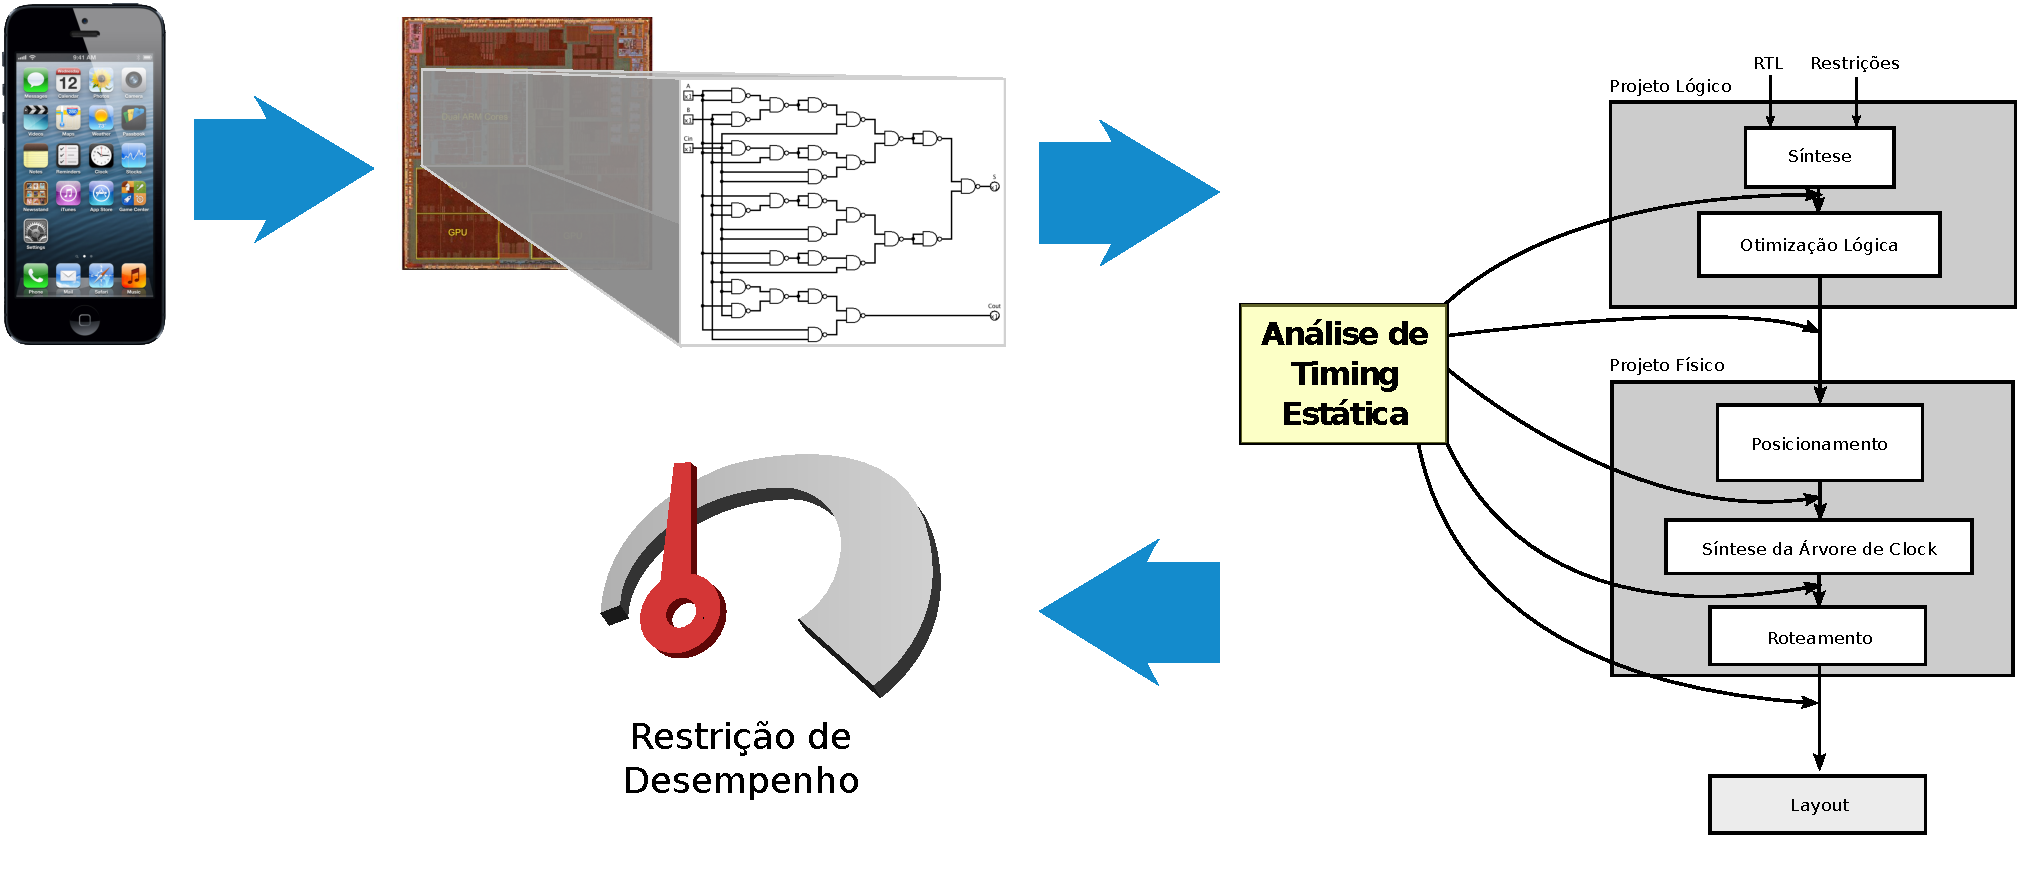
\includegraphics[width=1.05 \linewidth, trim=2cm 0 0 0]{img/motivacao.pdf} 
%				\end{center}
%					
%				\begin{itemize}
%					\item Necessidade de um \textit{time-to-market} curto;
%					\item Adoção do fluxo \textit{standard cell}.
%				\end{itemize}
%			\end{frame}
			\begin{frame}
				\frametitle{Motivação}
				\pgfdeclareimage[width=\linewidth]{motivacao1}{img/motivacao1.pdf}
				\pgfdeclareimage[width=\linewidth]{motivacao2}{img/motivacao2.pdf}
				\pgfdeclareimage[width=\linewidth]{motivacao3}{img/motivacao3.pdf}
				\pgfdeclareimage[width=\linewidth]{motivacao4}{img/motivacao4.pdf}
				\pgfdeclareimage[width=\linewidth]{motivacao5}{img/motivacao5.pdf}


				\pgfuseimage{motivacao1}<1>
				\pgfuseimage{motivacao2}<2>
				\pgfuseimage{motivacao3}<3>
				\pgfuseimage{motivacao4}<4>
				\pgfuseimage{motivacao5}<5>
				
			
			\end{frame}
			
		
			\begin{frame}
				\frametitle{Motivação: Fluxo \textit{Standard Cell}}
				\begin{minipage}{0.5 \textwidth}
					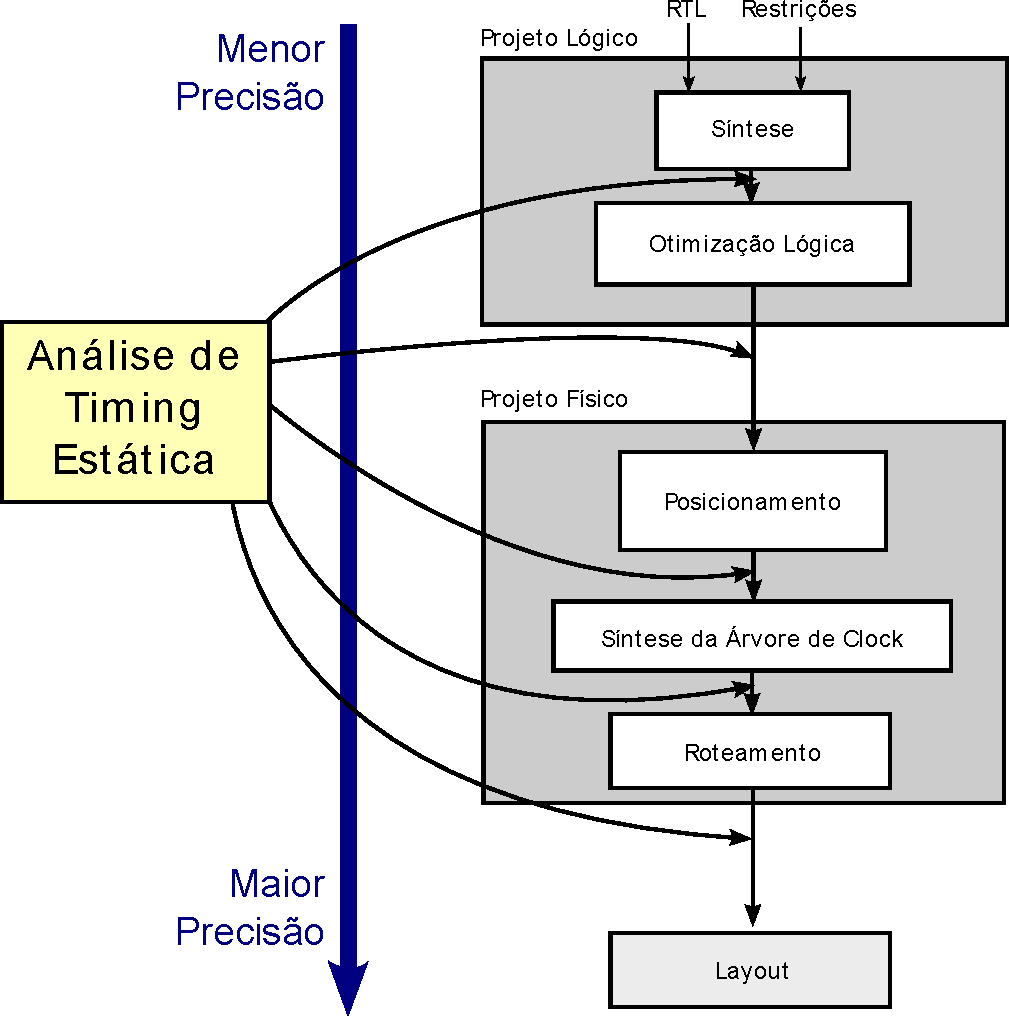
\includegraphics[width=\textwidth]{img/fluxo_standard_cell_sta_destacada.pdf}
				\end{minipage}
				\begin{minipage}{0.4 \textwidth}
					\begin{itemize}
						\item Diversas otimizações:
							\begin{itemize}
								\item Área;
								\item Potência;
								\item Atraso Máximo.
								
							\end{itemize}
						\item Avaliação das informações temporais durante o fluxo.
					\end{itemize}
				\end{minipage}
				
			\end{frame}
		
			\begin{frame}[t]
				\frametitle{Justificativa e Objetivos}
				\textbf{Justificativa:}
				\begin{itemize}
					\item Não se encontra na literatura uma validação extensa de uma técnica para cálculo do atraso de interconexões em circuitos de grande porte;					
					\item Inexistência de ferramentas de STA em domínio público;
					\item Alto custo das licenças das ferramentas industriais.
					
				\end{itemize}
				\pause
				\textbf{Objetivos:}
				\begin{itemize}
					\item Projeto, avaliação, validação e documentação de uma ferramenta de STA voltada para o fluxo \textit{standard cell;}
					\begin{enumerate}
						\item Modelo de interconexão de capacitância concentrada; \label{obj:1}
						\item Técnica de Elmore para cálculo dos atrasos das interconexões; \label{obj:2}
						\item Técnica para o cálculo do atraso das interconexões utilizando a abordagem de capacitância efetiva; \label{obj:3}
						\item Construção de uma ferramenta de STA que implementa \ref{obj:1}, \ref{obj:2} e \ref{obj:3}. 
					\end{enumerate}
				\end{itemize}
			\end{frame}
		
			
			\begin{frame}[t]
				\frametitle{Escopo}
				\begin{itemize}
					\item Modelos de atraso adotados em fluxo \textit{standard cell};
					\item 2 modelos de interconexão:
						\begin{enumerate}
							\item Modelo de Capacitância Concentrada;
							\item Modelo RC Concentrado.
						\end{enumerate}
					\item \textbf{NÃO} faz parte do escopo:
					\begin{itemize}
						\item Tempos de \textit{setup} e \textit{hold} das células sequenciais.
					\end{itemize}
				\end{itemize}
				
				
			\end{frame}
		
	
	\section{Conceitos}
		
		\begin{frame}
		\frametitle{Características Temporais dos Circuitos Digitais}
			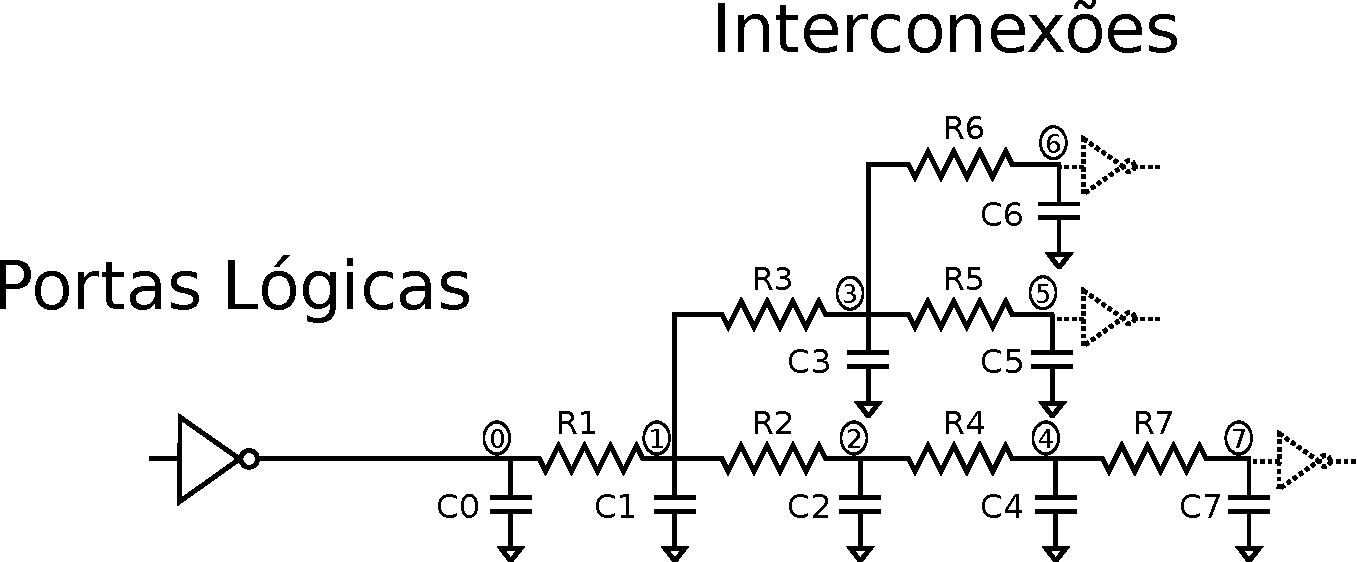
\includegraphics[width=\textwidth]{img/circuito.pdf} 
		\end{frame}

		\subsection*{Portas Lógicas}
			\begin{frame}
				\begin{center}
					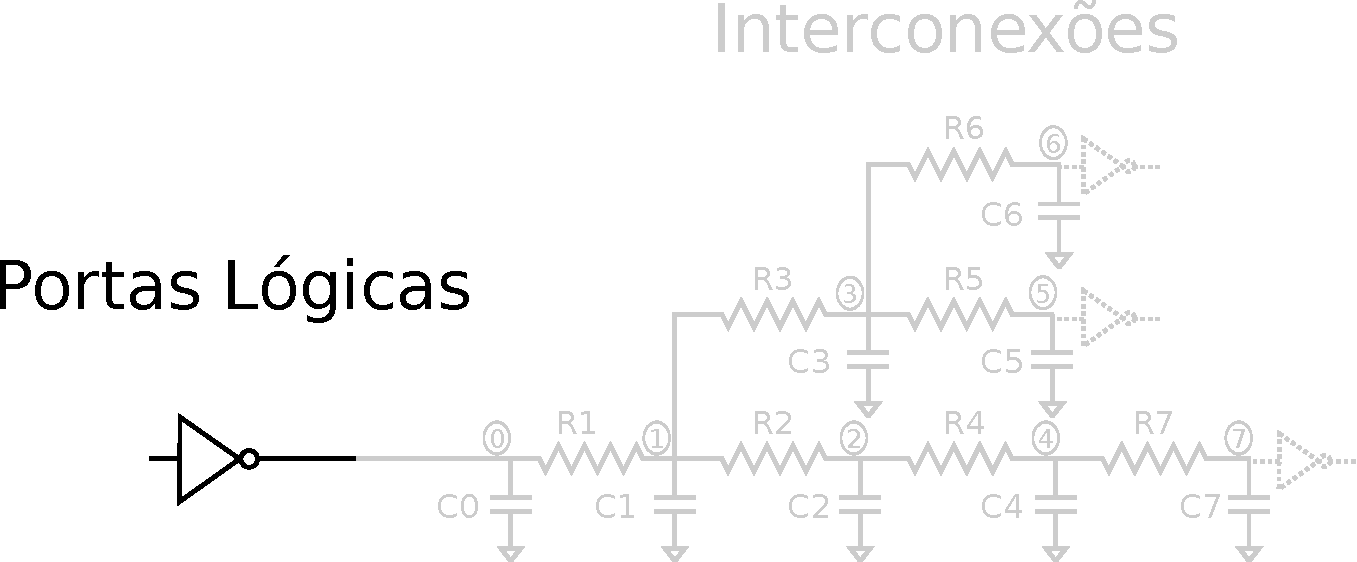
\includegraphics[width=\textwidth]{img/circuito_portas.pdf} 
				\end{center}
			\end{frame}
			
			\begin{frame}
				\frametitle{Características Temporais}
				\begin{itemize}
					\item \textit{Timing Arc} e \textit{Driver} \\
						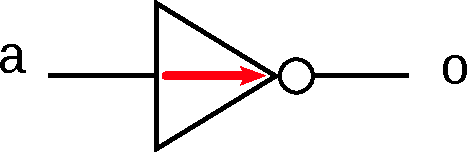
\includegraphics[width=0.3 \textwidth]{img/carac_portas_1.pdf}
					\item \textit{Delay} \\ 
						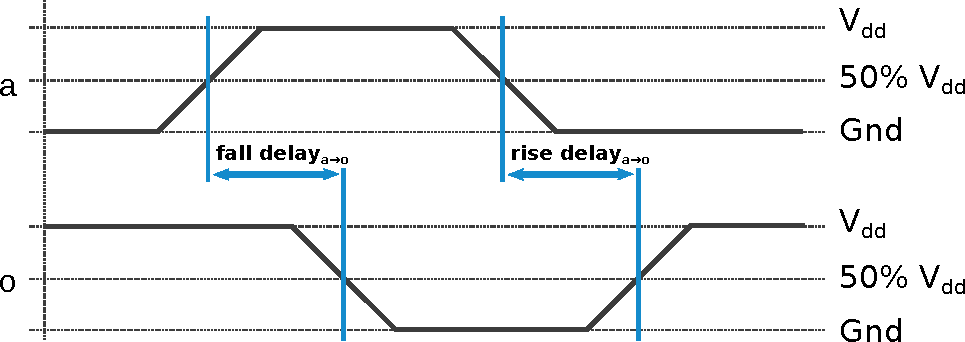
\includegraphics[width=0.7 \textwidth]{img/carac_portas_2.pdf} \pause
					\item \textit{Slew} \\
						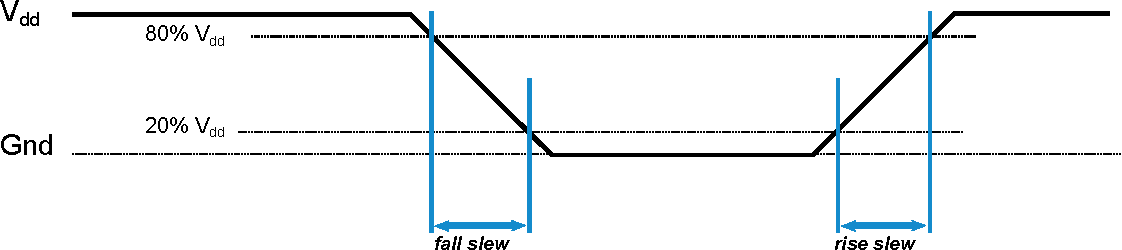
\includegraphics[width=0.7 \textwidth]{img/carac_portas_3.pdf}
				\end{itemize}

				
			\end{frame}

			
			\begin{frame}
				\frametitle{Modelo de Atraso Não-Linear}
					\begin{center}
						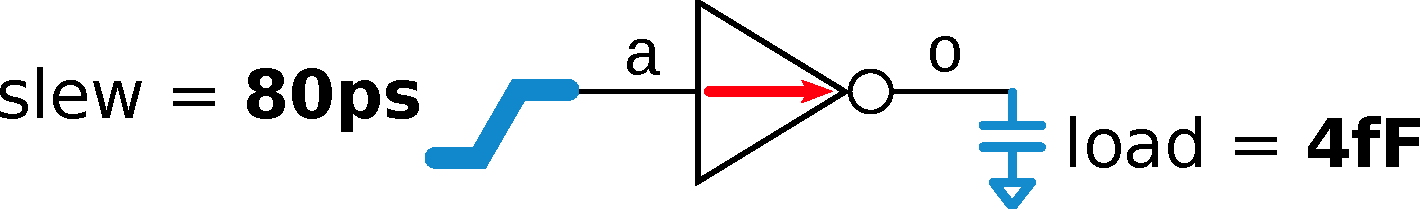
\includegraphics[width=0.7\textwidth]{img/nldm_1.pdf}
					\end{center}
					\begin{itemize}
						\item \textit{Delay}: $f(slew, load) = 52.05ps $	\\
						\begin{center}
							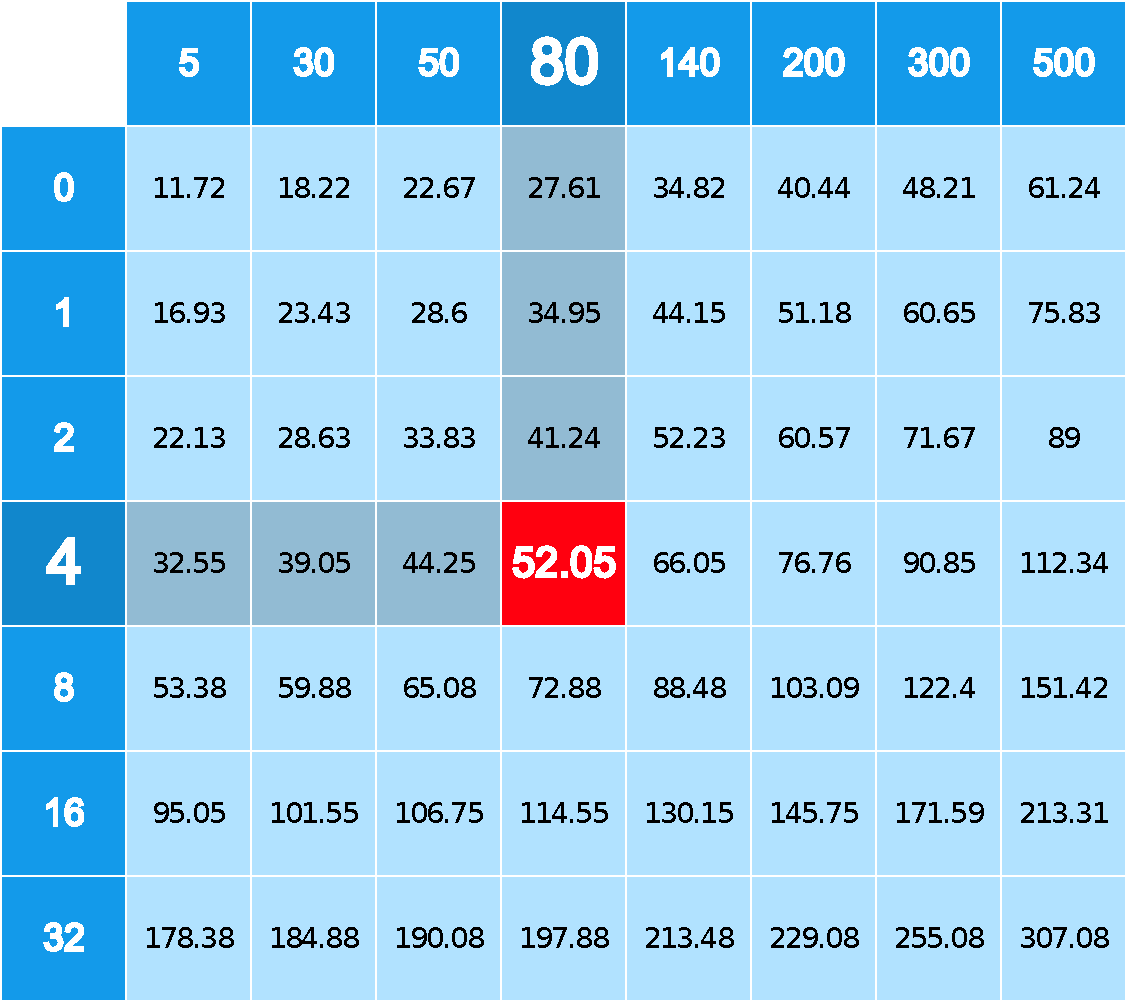
\includegraphics[width=0.4 \linewidth]{img/nldm_2.pdf} 
						\end{center}
					\end{itemize}					
						
			\end{frame}
		
		\subsection*{Interconexões}

			
			\begin{frame}
				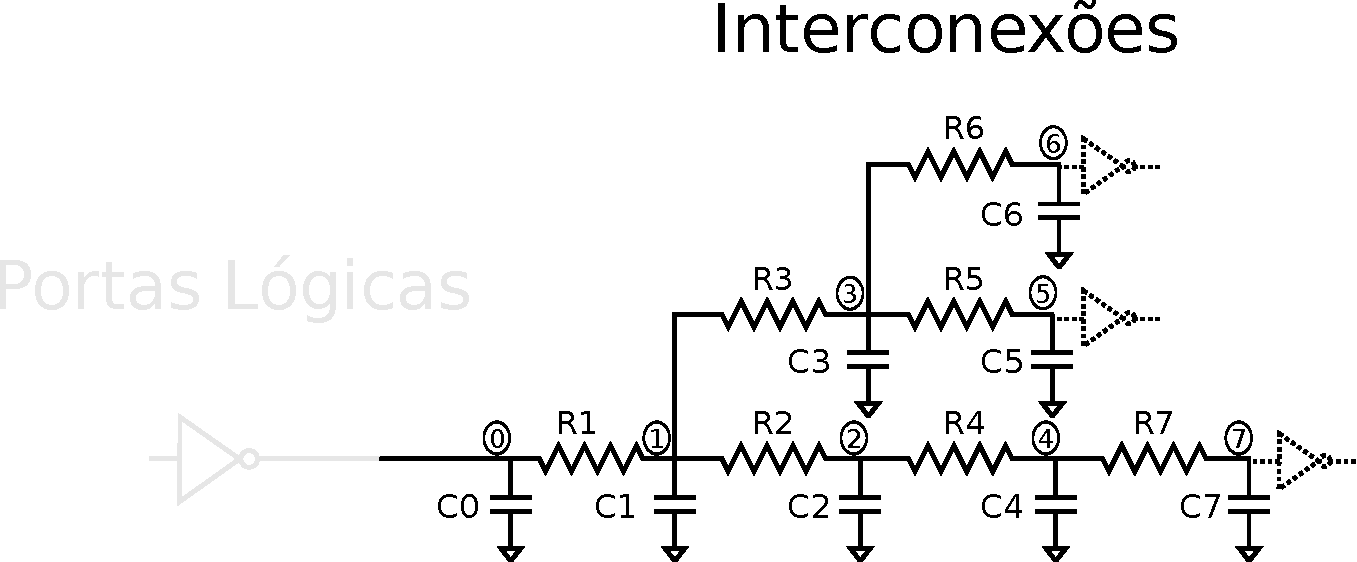
\includegraphics[width=\textwidth]{img/circuito_interconexao.pdf} 
			\end{frame}
			
			\subsubsection*{Características Temporais}
			\begin{frame}
				\frametitle{Características Temporais}
				
				
					\begin{figure}
						\subfigure
						{
						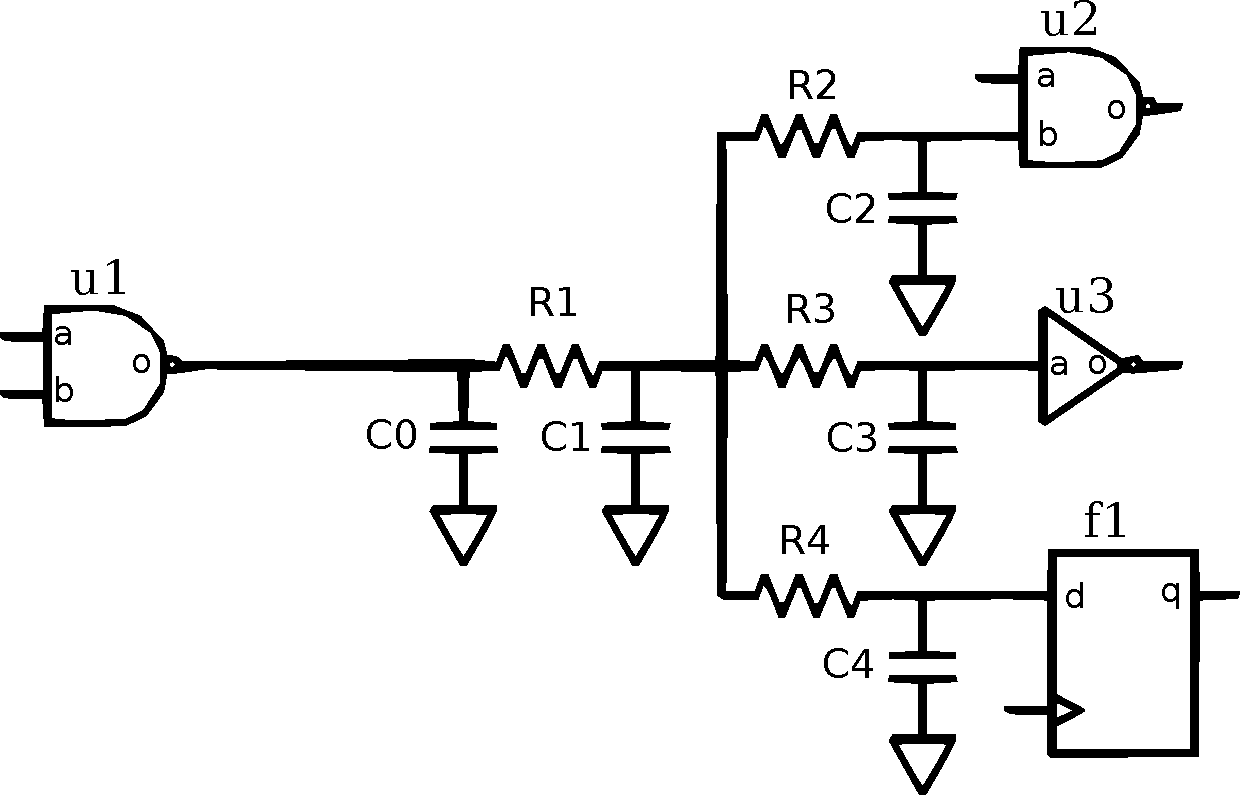
\includegraphics[width=0.4 \textwidth]{img/modelagem1.pdf}
						}
						\subfigure
						{
						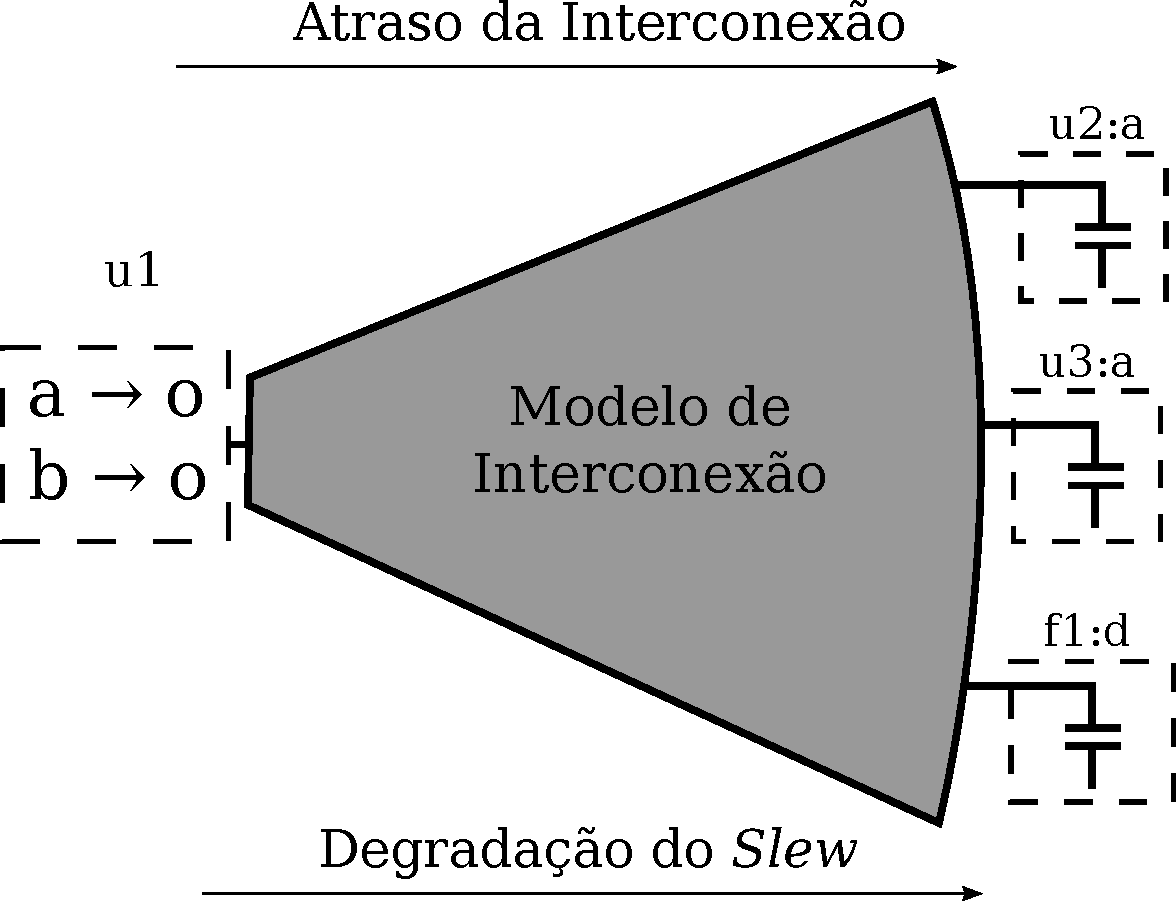
\includegraphics[width=0.4 \textwidth]{img/modelagem2.pdf}
						}
						
					\end{figure}
					\begin{itemize}
						\item Capacitância ``vista'' pelo \textit{driver};
						\item Atraso da interconexão;
						\item Degradação do \textit{slew}. 		
					\end{itemize}
			\end{frame}
			
			\subsubsection*{Modelos de Interconexões}
%				\begin{frame}
%					\frametitle{Modelo RC Distribuído}
%					\begin{center}
%						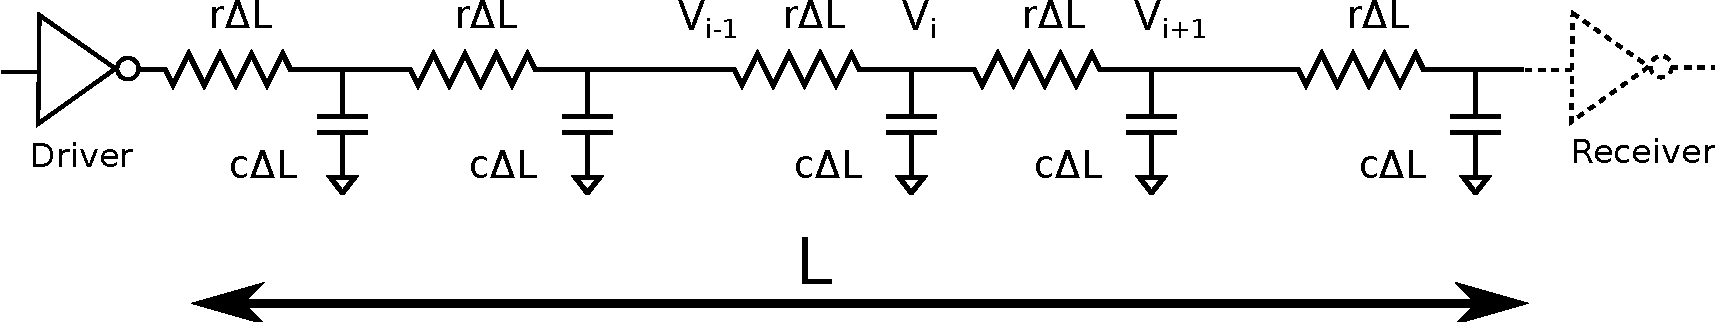
\includegraphics[width=\textwidth]{img/distributed_rc.pdf} 
%					\end{center}
%					\begin{itemize}
%						\item Cálculo do atraso reflete na solução de equações diferenciais (alto custo computacional);
%						\item Modelos de interconexão simplificados são mais adotados em fluxo \textit{standard cell}.
%					\end{itemize}
%					
%					
%				\end{frame}
				
				\begin{frame}
					\frametitle{Modelo de Capacitância Concentrada}
					\begin{center}
						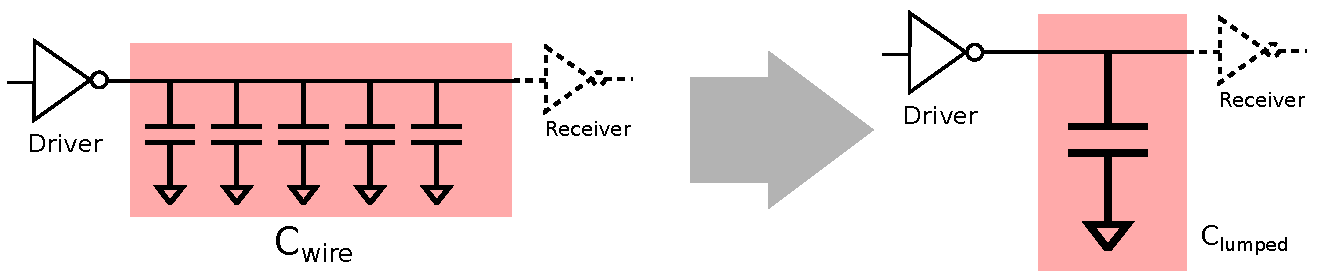
\includegraphics[width=\textwidth]{img/lumped_c.pdf} 
					\end{center}
					\begin{itemize}
						\item Amplamente utilizado nas primeiras etapas da síntese física;
						\item Modelo utilizado quando a resistência da interconexão é desprezível;
						\item Concentra-se toda a capacitância da interconexão em um único capacitor;
						\item O atraso da interconexão é desconsiderado.
					\end{itemize}							
				\end{frame}
				
				\begin{frame}
					\frametitle{Modelo de RC Concentrado}
					\begin{center}
						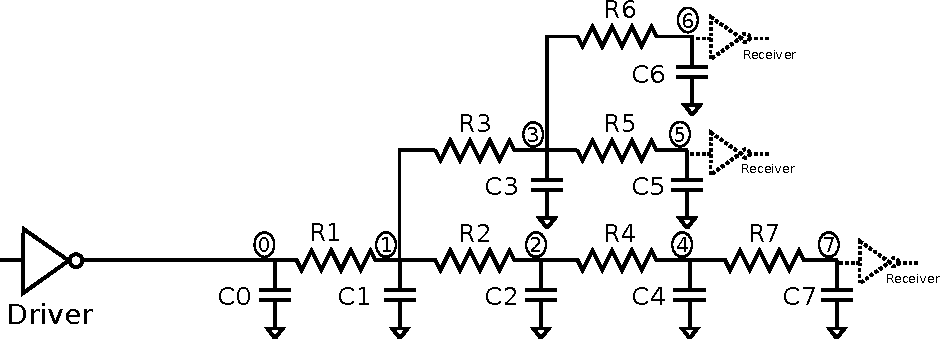
\includegraphics[width=\textwidth]{img/lumped_rc.pdf} 
					\end{center}
					\begin{itemize}
						\item Modelo amplamente adotado em fluxo \textit{standard cell};
						\item Concentra-se toda a resistência e capacitância de cada segmento em um único resistor R e capacitor C, respectivamente;
						\item Geralmente representado como uma árvore RC.
					\end{itemize}								
				\end{frame}
			
			
	
	\section{Trabalhos Correlatos}
		\subsection*{}
		\begin{frame}[t]
		\frametitle{Trabalhos Correlatos}
		
		\begin{columns}[t]
			\begin{column}{.6\linewidth}
				\pgfdeclareimage[width=\linewidth]{correlatos1}{img/correlatos1.pdf}
				\pgfdeclareimage[width=\linewidth]{correlatos2}{img/correlatos2.pdf}
				\pgfdeclareimage[width=\linewidth]{correlatos3}{img/correlatos3.pdf}
				\pgfdeclareimage[width=\linewidth]{correlatos4}{img/correlatos4.pdf}
				\pgfdeclareimage[width=\linewidth]{correlatos5}{img/correlatos5.pdf}
	
	
				\pgfuseimage{correlatos1}<1>
				\pgfuseimage{correlatos2}<2>
				\pgfuseimage{correlatos3}<3>
				\pgfuseimage{correlatos4}<4>
				\pgfuseimage{correlatos5}<5>
			\end{column}
			
			\begin{column}{.4\linewidth}
				\only<2>
				{
					\textbf{Kahng et. al. (2013)}
					\begin{itemize}
						\item Não utiliza capacitância efetiva;
						\item Erros superiores aos da técnica implementada neste trabalho.
					\end{itemize}
				}
				\only<3>
				{
					\begin{itemize}
						\item Modelos de alta ordem;
						\item Alto custo computacional.
					\end{itemize}
				}
				\only<4>
				{
					\begin{itemize}
						\item \textbf{Elmore Delay:} não considera o efeito de \textit{resistive shielding};
						\item \textbf{ECM:} aproxima o \textit{slew} do \textit{driver} da interconexão para obter o valor de capacitância efetiva.
					\end{itemize}
				}
				
				\only<5>
				{
					\begin{itemize}
						\item Técnica escolhida neste trabalho;
						\item Obtém o valor de \textit{slew} do \textit{driver} e capacitância efetiva iterativamente.
					\end{itemize}
				}
			\end{column}
			
			
			
		\end{columns}
		
			
		\end{frame}
	
	\section{Técnica Implementada}
	
		\subsection*{Visão Geral}
		
		\begin{frame}[t]
			\begin{center}
				\begin{columns}
					\begin{column}{0.63\textwidth}
						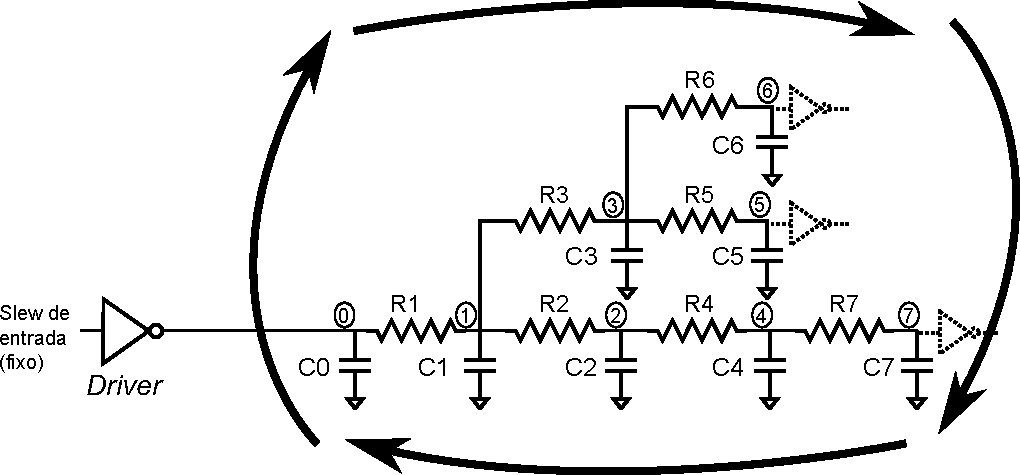
\includegraphics[width=\textwidth]{img/imagem_puri2.pdf} 
					\end{column}
					\begin{column}{0.37\textwidth}
						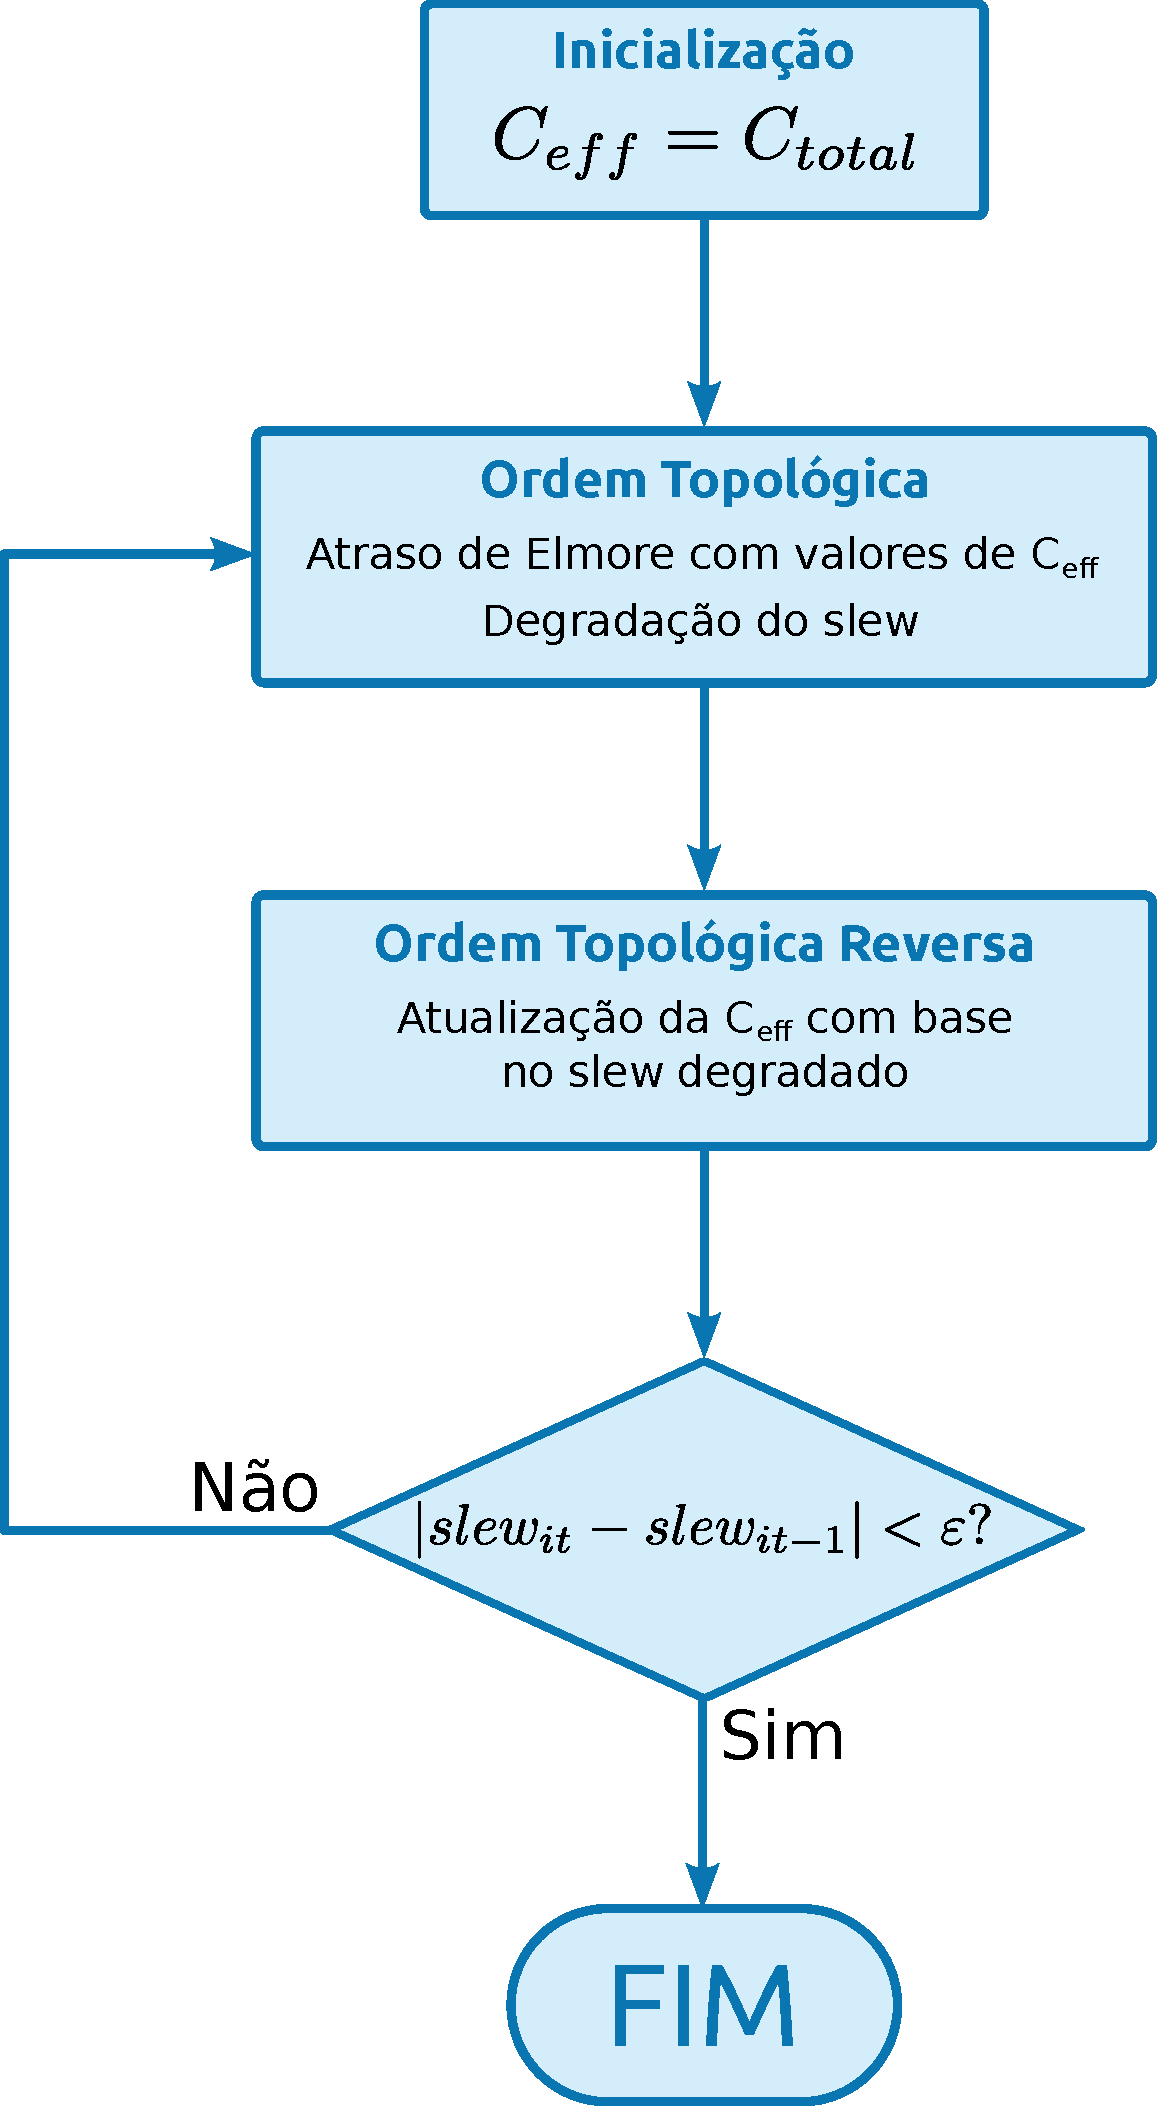
\includegraphics[width=\textwidth]{img/fluxograma.pdf} 
					\end{column}
				\end{columns}
			\end{center}
		\end{frame}


		\subsection*{Exemplo}

		\begin{frame}[t]
			\frametitle{Inicialização}
			\vspace{-0.25cm}
			\begin{center}
				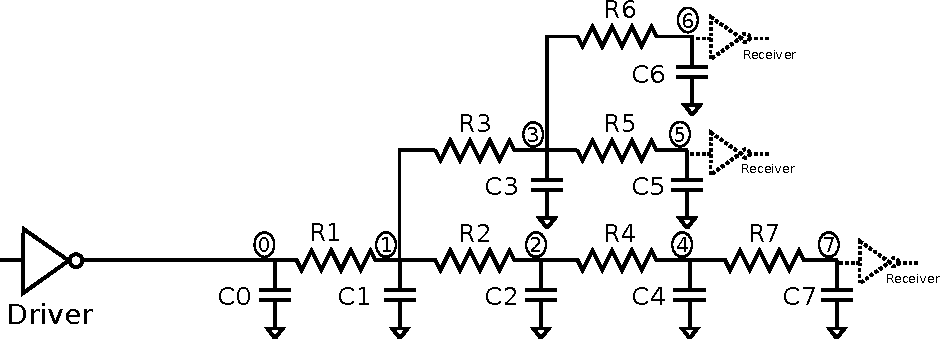
\includegraphics[width=0.8\linewidth]{img/inicializacao1.pdf}
			\end{center}
			\vspace{0.25cm}
			$C_{eff_0} = C_0 + C_1 + C_2 + C_3 + C_4 + C_5 + C_6 + C_7$ \\
			$C_{eff_1} = C_1 + C_2 + C_3 + C_4 + C_5 + C_6 + C_7$ \\
			$C_{eff_2} = C_2 + C_4 + C_7$ \\
			$C_{eff_3} = C_3 + C_5 + C_6$ \\
			$C_{eff_4} = C_4 + C_7$ \\
			$C_{eff_5} = C_5$ \\
			$C_{eff_6} = C_6$ \\
			$C_{eff_7} = C_7$
		\end{frame}


		\begin{frame}[t]
			\frametitle{Degradação dos \textit{Slews}}
			\pgfdeclareimage[width=\linewidth]{slew0}{img/slew0.pdf}
			\pgfdeclareimage[width=\linewidth]{slew1}{img/slew1.pdf}
			\pgfdeclareimage[width=\linewidth]{slew2}{img/slew2.pdf}
			\pgfdeclareimage[width=\linewidth]{slew22}{img/slew22.pdf}
			\pgfdeclareimage[width=\linewidth]{slew3}{img/slew3.pdf}
			

			\pgfuseimage{slew0}<1>
			\pgfuseimage{slew1}<2>
			\pgfuseimage{slew2}<3>
			\pgfuseimage{slew22}<4>
			\pgfuseimage{slew3}<5>
			
			\vspace{0.5cm}

			
			\only<1>{
				$\textcolor{azul}{slew_0} \gets slew\_biblioteca(C_{ceff_0})$			
			}
			
			\only<2>{
				\begin{columns}[t]
					\begin{column} {.35 \textwidth}
						$\textcolor{vermelho}{slew_1} \gets \frac{\textcolor{azul}{slew_0}}{1 - x(1 - e^{-\frac{1}{x}})}$\\\vspace{0.25cm}
						$x = \frac{R_1 C_{eff_1}}{\textcolor{azul}{slew_0}}$
					\end{column}
					\begin{column} {.65 \textwidth}
						\begin{itemize}
							\item Resposta ao impulso do nodo 1 em relação ao nodo 0;
						\end{itemize}
					\end{column}
				\end{columns}
			}
			\only<3>{
				$\textcolor{vermelho}{slew_3} \gets \frac{\textcolor{azul}{slew_1}}{1 - x(1 - e^{-\frac{1}{x}})}$\\\vspace{0.25cm}
				$x = \frac{R_3 C_{eff_3}}{\textcolor{azul}{slew_1}}$
			}
			\only<4>{
				$\textcolor{vermelho}{slew_2} \gets \frac{\textcolor{azul}{slew_1}}{1 - x(1 - e^{-\frac{1}{x}})}$\\\vspace{0.25cm}
				$x = \frac{R_2 C_{eff_2}}{\textcolor{azul}{slew_1}}$
			}
			\only<5>{
				\textbf{[...]}\\
				\begin{columns}[t]
			
					\begin{column}{0.33 \textwidth}
						$\textcolor{vermelho}{slew_5} \gets \frac{slew_3}{1 - x_5(1 - e^{-\frac{1}{x_5}})}$
					\end{column}
					\begin{column}{0.33 \textwidth}
						$\textcolor{vermelho}{slew_6} \gets \frac{slew_3}{1 - x_6(1 - e^{-\frac{1}{x_6}})}$
					\end{column}
					\begin{column}{0.33 \textwidth}
						$\textcolor{vermelho}{slew_7} \gets \frac{slew_4}{1 - x_7(1 - e^{-\frac{1}{x_7}})}$
					\end{column}
				\end{columns}
%				$\textcolor{vermelho}{slew_5} \gets \frac{slew_3}{1 - x_5(1 - e^{-\frac{1}{x_5}})}$\\
%				$\textcolor{vermelho}{slew_6} \gets \frac{slew_3}{1 - x_6(1 - e^{-\frac{1}{x_6}})}$\\
%				$\textcolor{vermelho}{slew_7} \gets \frac{slew_4}{1 - x_7(1 - e^{-\frac{1}{x_7}})}$\\

			}

		\end{frame}

		\begin{frame}[t]
			\frametitle{Atualização da Capacitância Efetiva}
%			\begin{minipage}{\linewidth}
			\pgfdeclareimage[width=\linewidth]{inicializacao2}{img/inicializacao2.pdf}
			\pgfdeclareimage[width=\linewidth]{inicializacao3}{img/inicializacao3.pdf}
			\pgfdeclareimage[width=\linewidth]{inicializacao4}{img/inicializacao4.pdf}
			\pgfdeclareimage[width=\linewidth]{inicializacao5}{img/inicializacao5.pdf}
			\pgfdeclareimage[width=\linewidth]{inicializacao6}{img/inicializacao6.pdf}
			\pgfdeclareimage[width=\linewidth]{inicializacao7}{img/inicializacao7.pdf}


			\pgfuseimage{inicializacao2}<1>
			\pgfuseimage{inicializacao3}<2>
			\pgfuseimage{inicializacao4}<3>
			\pgfuseimage{inicializacao5}<4>
			\pgfuseimage{inicializacao6}<5>
			\pgfuseimage{inicializacao7}<6>
			
			\vspace{0.5cm}
				
%			\end{minipage}
			\only<1>{
				$C_{eff_7} \gets \textcolor{verde}{C_7}$\\
				$C_{eff_6} \gets \textcolor{verde}{C_6}$\\
				$C_{eff_5} \gets \textcolor{verde}{C_5}$
			}
			
					
			\only<2-3>{
				\begin{columns}
					\begin{column}{.4\linewidth}
						$C_{eff_4} \gets \textcolor{verde}{C_4}$
						\only<3>{
							$\textcolor{azul}{+ C_{eff_7} \times K_7}$ \\\vspace{0.25cm}
							$K_7 = 1 - \frac{2 R_7 C_{eff_7}}{slew_4}(1 - e^{-\frac{slew_4}{2 R_7 C_{eff_7}}})$
						}
					\end{column}
					\begin{column}{.6\linewidth}
						\begin{itemize}
							\item $K_7 \in [0, 1]$;
							\item $\uparrow K_7 \downarrow$ Resistive Shielding.
						\end{itemize}
					\end{column}
				\end{columns}
			}
			\only<4-5>{
				$C_{eff_3} \gets \textcolor{verde}{C_3}$
				\only<5>{
					$\textcolor{azul}{+ C_{eff_5} \times K_5 + C_{eff_6} \times K_6}$ \\\vspace{0.25cm}
					$K_5 = 1 - \frac{2 R_5 C_{eff_5}}{slew_3}(1 - e^{-\frac{slew_3}{2 R_5 C_{eff_5}}})$\\
					$K_6 = 1 - \frac{2 R_6 C_{eff_6}}{slew_3}(1 - e^{-\frac{slew_3}{2 R_6 C_{eff_6}}})$
				}
			}
			\only<6>{
				\textbf{[...]} \\\vspace{0.25cm}
				$C_{eff_0} \gets \textcolor{verde}{C_0} \textcolor{azul}{+ C_{eff_1} \times K_1}$\\\vspace{0.25cm}
				$K_1 = 1 - \frac{2 R_1 C_{eff_1}}{slew_0}(1 - e^{-\frac{slew_0}{2 R_1 C_{eff_1}}})$
			}
			
			
							
		\end{frame}
	
	\section{Análise de Timing Estática}
	
		\subsection*{}
		\begin{frame}
			\frametitle{Análise de \textit{Timing} Estática}
			\pgfdeclareimage[width=0.8\linewidth]{circuitinho1}{img/circuitinho.pdf}
			\pgfdeclareimage[width=0.8\linewidth]{circuitinho2}{img/circuitinho_contexto_interconexao.pdf}
			\pgfdeclareimage[width=0.8\linewidth]{circuitinho3}{img/circuitinho_contexto_caminhos.pdf}
			\begin{center}
				\pgfuseimage{circuitinho1}<1>
				\pgfuseimage{circuitinho2}<2>
				\pgfuseimage{circuitinho3}<3>
			\end{center}
		\end{frame}
		
		\begin{frame}[t]
			\frametitle{Visão Geral}
			\begin{center}
				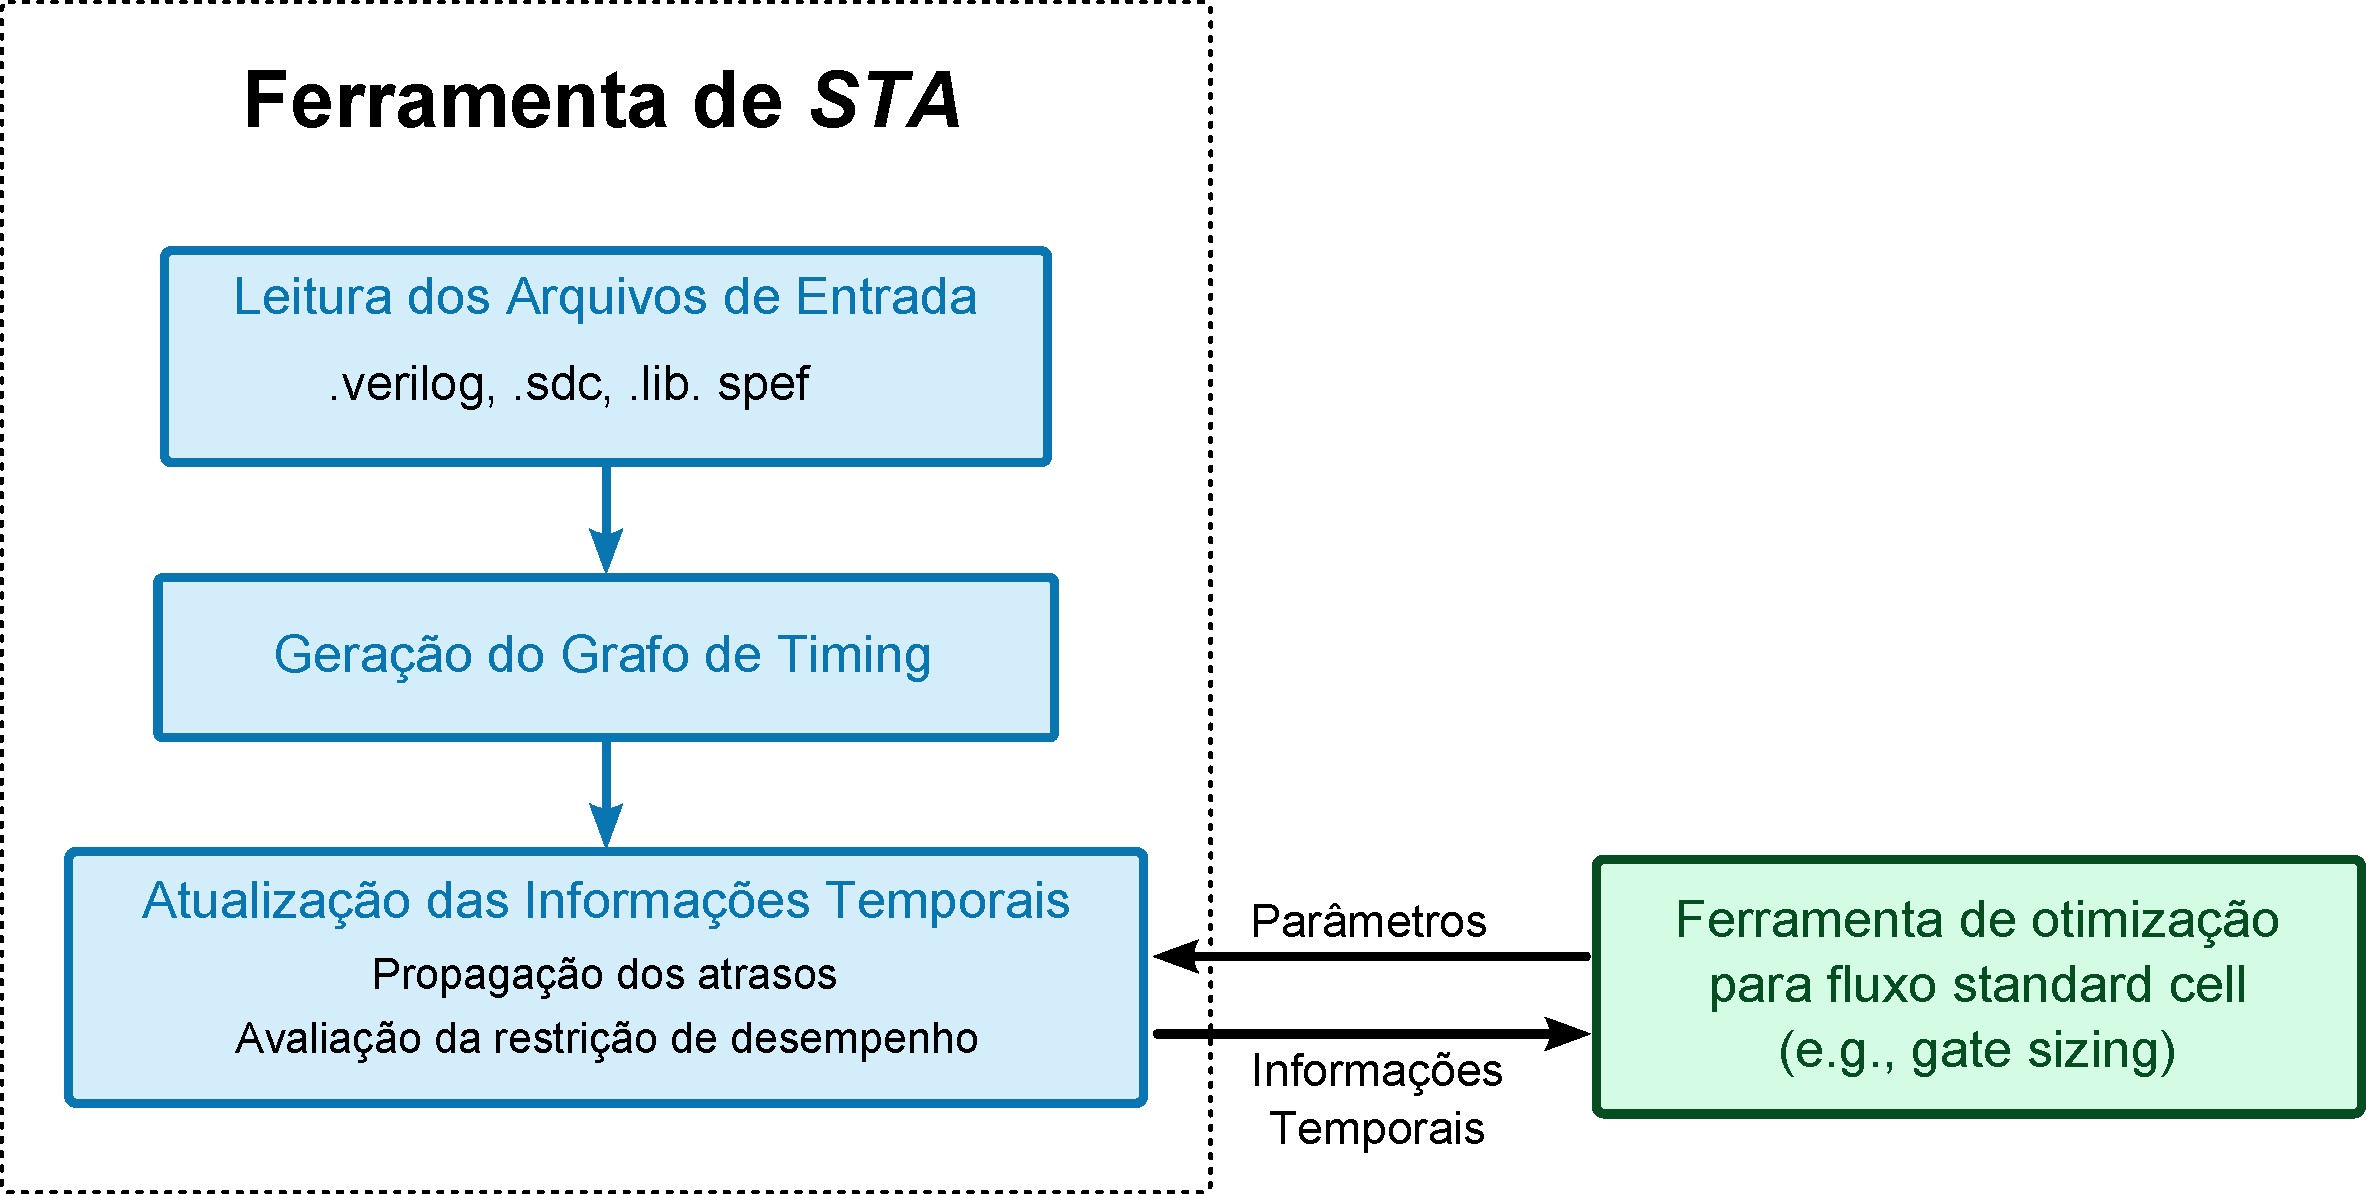
\includegraphics[width=\linewidth]{img/fluxograma_sta.pdf}
			\end{center}
		\end{frame}
		
		\begin{frame}[t]
			\frametitle{Grafo de \textit{Timing}}
			\begin{center}
				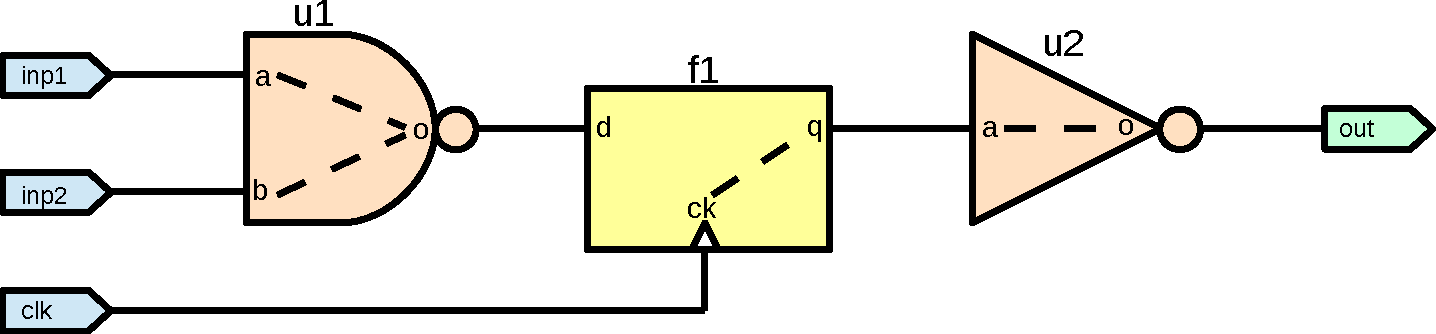
\includegraphics[width=0.7\linewidth]{img/exemplo_circuito_simple.pdf} \\\vspace{0.5cm} 
				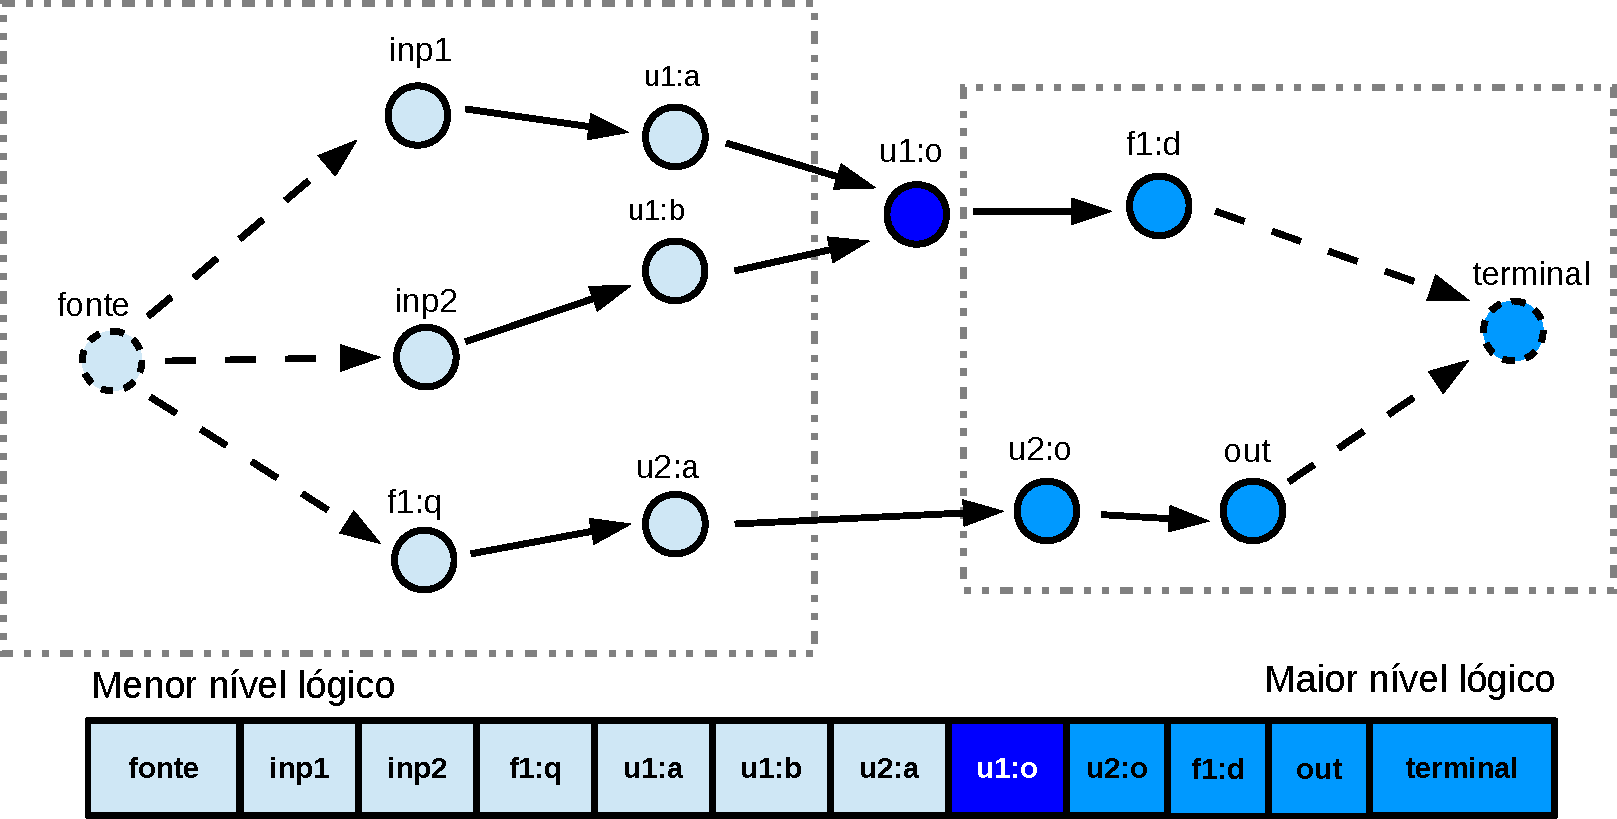
\includegraphics[width=0.8\linewidth]{img/grafo_lista_nivel_logico.pdf}
			\end{center}
		\end{frame}
%		\begin{frame}[t]
%			\frametitle{Algoritmo de STA}
%			\begin{algorithm}[H]
%				\ParaTodo{ $v_i \in V$ em ordem topológica}{
%					\uSe{$v_i$ é um pino de entrada}
%					{
%						Cálculo da $C_{eff}$;\\
%						Cálculo do \textit{delay} e \textit{slew};\\
%						Propagação do \textit{arrival time}.
%					}
%					\SenaoSe{$v_i$ é um pino de saída ou é uma entrada primária}
%					{
%						Propagação do \textit{arrival time} pela interconexão.
%					}
%				}
%				\ParaTodo{ $v_i \in V$ em ordem topológica reversa}{
%					Atualização das folgas.
%				}
%			\end{algorithm}
%		\end{frame}
		\begin{frame}
			\frametitle{Exemplo}
			\pgfdeclareimage[width=0.8\linewidth]{algoritmo1}{img/algoritmo1.pdf}
			\pgfdeclareimage[width=0.8\linewidth]{algoritmo2}{img/algoritmo2.pdf}
			\pgfdeclareimage[width=0.8\linewidth]{algoritmo3}{img/algoritmo3.pdf}
			\pgfdeclareimage[width=0.8\linewidth]{algoritmo4}{img/algoritmo4.pdf}
			\pgfdeclareimage[width=0.8\linewidth]{algoritmo5}{img/algoritmo5.pdf}
			\pgfdeclareimage[width=0.8\linewidth]{algoritmo6}{img/algoritmo6.pdf}
			\pgfdeclareimage[width=0.8\linewidth]{algoritmo7}{img/algoritmo7.pdf}
			\pgfdeclareimage[width=0.8\linewidth]{algoritmo8}{img/algoritmo8.pdf}

			\begin{center}
				\pgfuseimage{algoritmo1}<1>
				\pgfuseimage{algoritmo2}<2>
				\pgfuseimage{algoritmo3}<3>
				\pgfuseimage{algoritmo4}<4>
				\pgfuseimage{algoritmo5}<5>
				\pgfuseimage{algoritmo6}<6>
				\pgfuseimage{algoritmo7}<7>
				\pgfuseimage{algoritmo8}<8>
			\end{center}

		\end{frame}
	
	\section{Experimentos}
		
		\subsection*{}
		\begin{frame}
			\frametitle{Metodologia Experimental}
			\begin{center}
				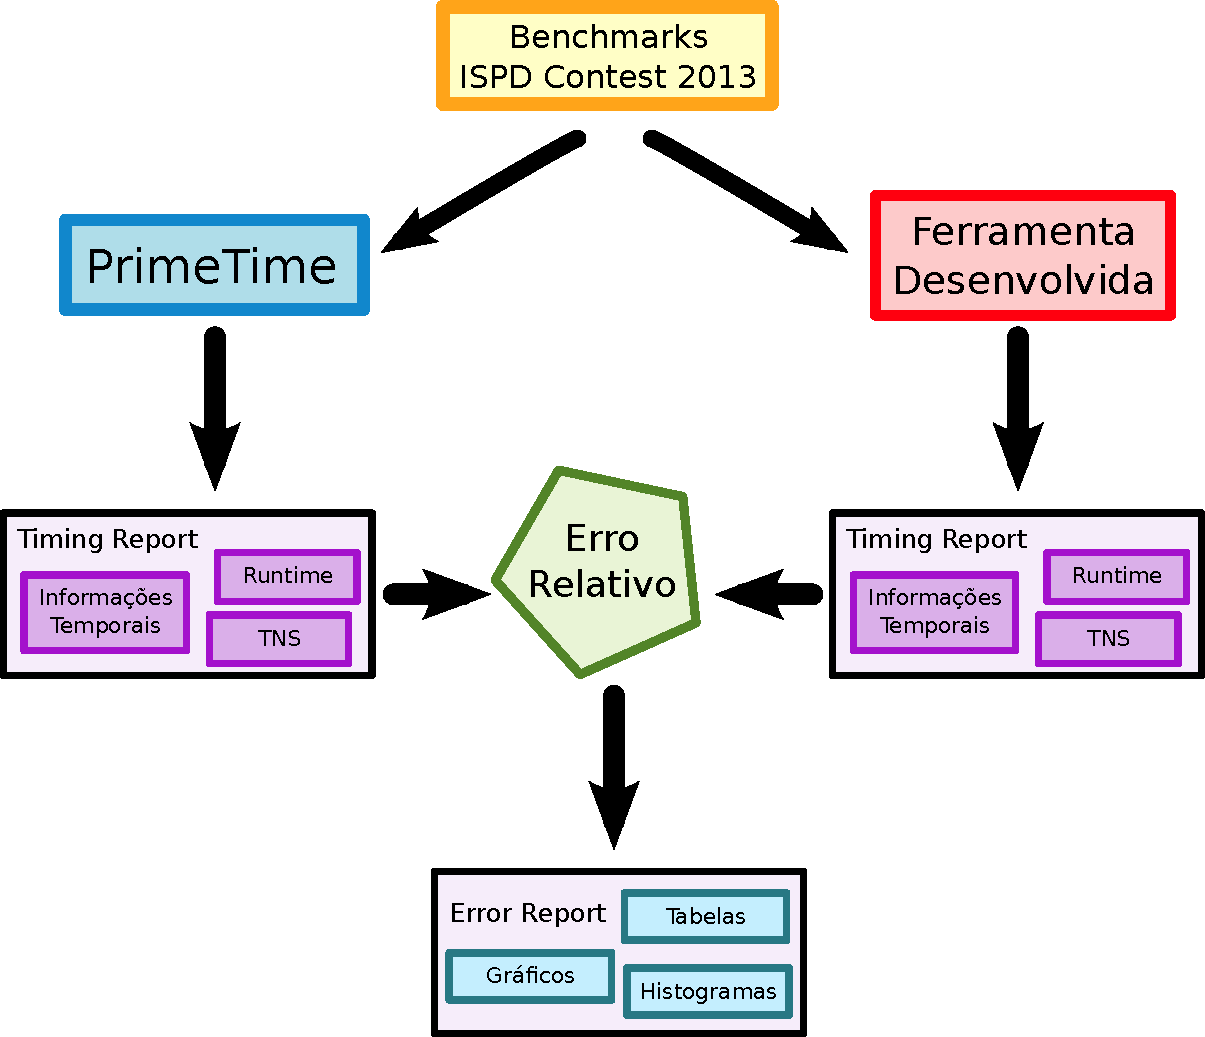
\includegraphics[width=0.75\linewidth]{img/fluxo_validacao.pdf} 
			\end{center}	
		\end{frame}	
		
		\begin{frame}[t]
			\frametitle{Metodologia e Infraestrutura Experimental}
			\begin{center}
				\begin{itemize}
					\item \textbf{Técnicas que foram comparadas ferramenta industrial:}	\\
						\begin{itemize}
							\item Capacitância concentrada \textbf{SEM} atraso de interconexões;
							\item Capacitância efetiva \textbf{COM} atraso de interconexões \textbf{E} degradação do \textit{slew}.							
							\item Capacitância concentrada \textbf{COM} atraso de Elmore para interconexões \textbf{E} degradação do \textit{slew};
							
						\end{itemize} \pause
					\item \textbf{Infraestrutura Experimental: } \\
						\begin{itemize}
						\item 8 circuitos (608-982k portas lógicas): \\
						\begin{itemize}
							\item Descrição em linguagem de descrição de \textit{hardware} (.v); \\
							\item Restrições de projeto (.sdc);\\
							\item Descrição dos parasitas RC (.spef).
						\end{itemize}
						\item Biblioteca \textit{standard cell} realista; \\
					\end{itemize} 
				\end{itemize}
				
			\end{center}
		\end{frame}			
		
		\subsection*{Experimentos}
		\begin{frame}[t]
			\frametitle{Validação do Modelo de Capacitância Concentrada}
			\vspace{-.5cm}
			\begin{center}
				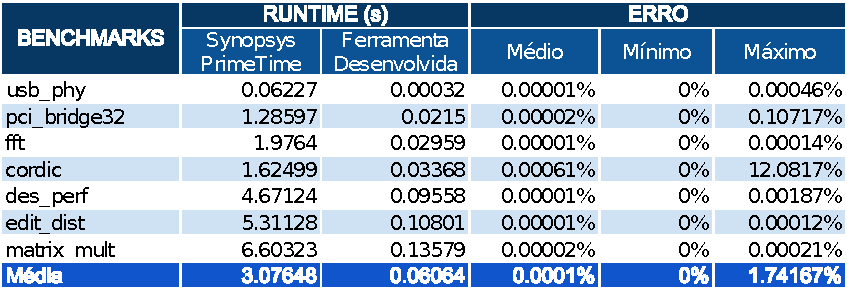
\includegraphics[width=0.9\linewidth]{img/lumped_capacitance_vs_primetime.pdf} 
			\end{center}
			\vspace{-.5cm}
			\begin{columns}
				\begin{column}{0.4\textwidth}
					\begin{shaded}
						$erro = 100 \times \frac{a - b}{ b } $ \\
						\small{a = ferramenta implementada} \\
						\small{b = primetime}
					\end{shaded}
				\end{column}
				\begin{column}{0.6\textwidth}
					\begin{itemize}
						\item \textbf{0\%} de erro;
						\item Ferramenta cerca de \textbf{50x mais rápida} nos 7 primeiros circuitos;
						\item \textbf{6.19x mais rápida} no netcard.
					\end{itemize}
				\end{column}
			\end{columns}
			
			
		\end{frame}
		
		
		%PURI
		\begin{frame}[t]
			\frametitle{$C_{eff}$ + atraso da interconexão + degradação do \textit{slew}}
			\vspace{-.5cm}
			\begin{center}
				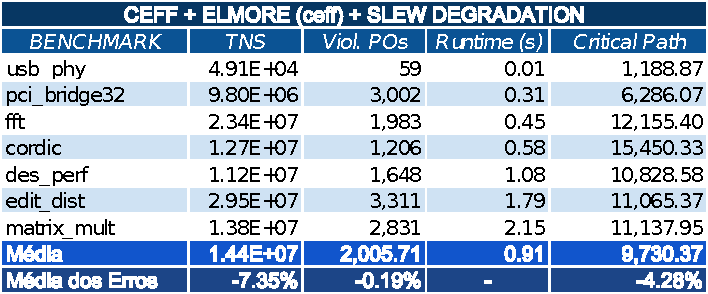
\includegraphics[width=0.9\linewidth]{img/ceff_elmore_slew.pdf}
			\end{center}
			\vspace{-.5cm}
			\begin{columns}
				\begin{column}{0.4\textwidth}
					\begin{shaded}
						$erro = 100 \times \frac{a - b}{ b } $ \\
						\small{a = ferramenta implementada} \\
						\small{b = primetime}
					\end{shaded}
				\end{column}
				\begin{column}{0.6\textwidth}
					\begin{itemize}
						\item Média dos erros \textbf{baixa} (\textbf{-8.52\%} e \textbf{-4.16\%});
						\item Resultados otimistas.
						\item Cerca de \textbf{8x mais rápida};
					\end{itemize}
				\end{column}
			\end{columns}			
			
		\end{frame}
		
		% ERRO POS
%		\begin{frame}[t]
%			\frametitle{Erros de \textit{arrival} nas saídas primárias}
%			\begin{itemize}
%				\item Circuito $pci\_bridge32\_slow$ (31k portas lógicas);
%			\end{itemize}
%			\begin{center}
%				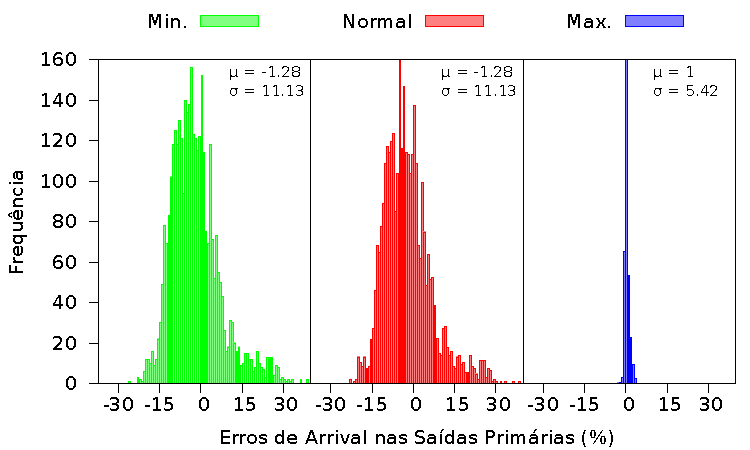
\includegraphics[width=0.9\linewidth]{img/arrival_error/pci_bridge32_puri.pdf}\\
%			\end{center}
%		\end{frame}		
%		
		\begin{frame}[t]
			\frametitle{Erros de \textit{arrival} nas saídas primárias}
			\begin{itemize}
				\item Circuito $matrix\_mult\_slow$ (156k portas lógicas);
			\end{itemize}
			\begin{center}
				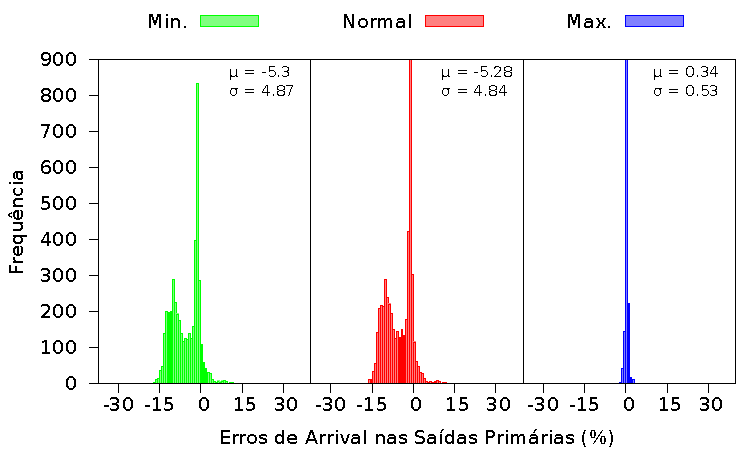
\includegraphics[width=0.8\linewidth]{img/arrival_error/matrix_mult_puri.pdf}\\
			\end{center}
			\vspace{-.6cm}
			\begin{columns}
					\begin{column}{0.4 \textwidth}
						\begin{shaded}
							\scriptsize{\textbf{Min.:} Portas com menor desempenho;} \\
							\scriptsize{\textbf{Normal:} Configuração padrão;}\\
							\scriptsize{\textbf{Max.:} Portas com maior desempenho.}
						\end{shaded}
					\end{column}
					\begin{column}{0.6 \textwidth}
						\begin{itemize}
							\item Maior desempenho $\to C_{eff} \approx C_{total}$.
						\end{itemize}
					\end{column}
				\end{columns}			
		\end{frame}
		
		%NO SLEW
		\begin{frame}[t]
			\frametitle{Impacto da degradação do \textit{slew}}
			\vspace{-.5cm}
			\begin{center}
				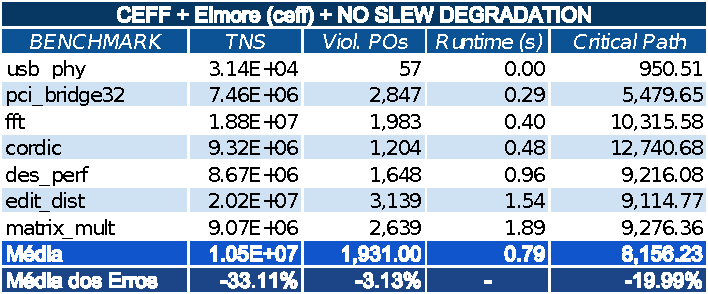
\includegraphics[width=\linewidth]{img/ceff_elmore_no_slew.pdf}
			\end{center}
			\vspace{-.5cm}
			\begin{columns}
				\begin{column}{0.4\textwidth}
					\begin{shaded}
						$erro = 100 \times \frac{a - b}{ b } $ \\
						\small{a = ferramenta implementada} \\
						\small{b = primetime}
					\end{shaded}
				\end{column}
				\begin{column}{0.6\textwidth}
					\begin{itemize}
						\item Média dos erros \textbf{muito} alta (\textbf{-40.79\%} e \textbf{-19.41\%});
						\item Resultados \textbf{muito} otimistas.
					\end{itemize}
				\end{column}
			\end{columns}	
			
		\end{frame}
		
		
		% CEFF / CTOTAL
		\begin{frame}[t]
			\frametitle{Relação $C_{eff} / C_{total}$}
			\begin{center}
				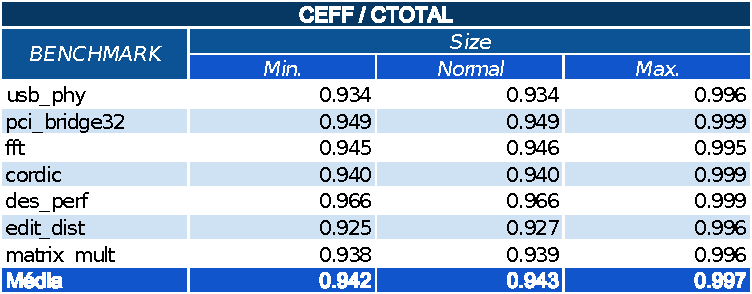
\includegraphics[width=0.9\linewidth]{img/ceff_ratio/ceff_ctotal_todos.pdf}
				\begin{columns}
					\begin{column}{0.4 \textwidth}
						\begin{shaded}
							\scriptsize{\textbf{Min.:} Portas com menor desempenho;} \\
							\scriptsize{\textbf{Normal:} Configuração padrão;}\\
							\scriptsize{\textbf{Max.:} Portas com maior desempenho.}
						\end{shaded}
					\end{column}
					\begin{column}{0.6 \textwidth}
						\begin{itemize}
							\item Maior desempenho $\to C_{eff} \approx C_{total}$.
						\end{itemize}
					\end{column}
				\end{columns}						
			\end{center}
			
		\end{frame}
		
%		\begin{frame}
%			\frametitle{Relação $C_{eff} / C_{total}$: $pci\_bridge32\_slow$}
%			\begin{center}
%				\pgfdeclareimage[width=0.9\linewidth]{ratiopci}{img/experimentos/pcifull.pdf}
%				\pgfdeclareimage[width=0.9\linewidth]{ratiopcizoom}{img/experimentos/pcizoom.pdf}
%				\pgfuseimage{ratiopci}<1>
%				\pgfuseimage{ratiopcizoom}<2>
%			\end{center}
%			
%			\only<2>
%			{
%				\begin{itemize}
%					\item Maior resistência $\to$ Maior \textit{shielding};
%				\end{itemize}
%			}
%		\end{frame}
		
		\begin{frame}
			\frametitle{Relação $C_{eff} / C_{total}$}
			\begin{itemize}
				\item Circuito $matrix\_mult\_slow$ (156k portas lógicas).
			\end{itemize}
			\begin{center}
				\pgfdeclareimage[width=0.9\linewidth]{ratiomatrix}{img/experimentos/matrixfull.pdf}
				\pgfuseimage{ratiomatrix}<1>
			\end{center}

			\begin{itemize}
				\item Maior resistência $\to$ Maior \textit{shielding};
			\end{itemize}
		\end{frame}

		% LUMPED
		\begin{frame}[t]
			\frametitle{$C_{total}$ + atraso da interconexão + degradação do \textit{slew}}
			\vspace{-.5cm}
			\begin{center}
				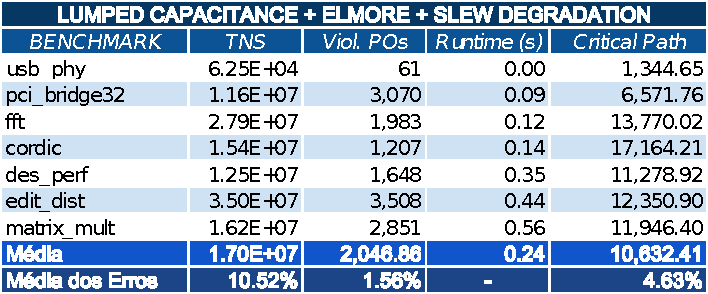
\includegraphics[width=\linewidth]{img/lump_elmore_slew.pdf}
			\end{center}
%			\vspace{-.5cm}
			\begin{columns}
				\begin{column}{0.4\textwidth}
					\begin{shaded}
						$erro = 100 \times \frac{a - b}{ b } $ \\
						\small{a = ferramenta implementada} \\
						\small{b = primetime}
					\end{shaded}
				\end{column}
				\begin{column}{0.6\textwidth}
					\begin{small}
					
						\begin{itemize}
							\item Erro \textbf{baixo} para TNS nos 7 primeiros circuitos (\textbf{10.52\%});
							\item Erro \textbf{baixo} para \textit{critical path} (\textbf{5.11\%});
							\item Resultados pessimistas;
							\item Cerca de \textbf{32x mais rápida};
						\end{itemize}
					\end{small}
				\end{column}
			\end{columns}			
			
		\end{frame}
		
		
		
	
	\section{Conclusões}
	
		\begin{frame}[t]
		\frametitle{Conclusões}
			\begin{itemize}
				\item Foram avaliados os impactos do atraso das interconexões e degradação dos \textit{slews} no contexto de uma ferramenta de análise de \textit{timing} estática;			
			
				\item A desconsideração da degradação do \textit{slew} pode levar a uma estimativa muito otimista (mais de 40\% de erro);
				
				\item Capacitância Efetiva $\to$ \textit{Resistive Shielding};
				
				\item A ferramenta implementada é otimista em relação ao \textit{PrimeTime} em \textbf{4.16\%} na média, com tempo de execução  cerca de \textbf{8x} menor;
				
				\item $C_{eff} / C_{total} \approx 1$ nos circuitos da competição do ISPD 2013.
				
				\item Abordagem de capacitância concentrada + Elmore + Degradação do \textit{slew} é \textbf{pessimista} em relação ao \textit{PrimeTime} em \textbf{5.11\%} na média, com tempo de execução cerca de \textbf{32x} menor.
			\end{itemize}
		\end{frame}
	
%	\section{Trabalhos Futuros}
%		
%		\begin{frame}[t]
%		\frametitle{Trabalhos Futuros}
%			\begin{itemize}
%				\item Investigação detalhada dos erros obtidos;
%				
%				\item Avaliação da técnica de STA em uma ferramenta de otimização (e.g., \textit{gate sizing});
%				
%				\item Utilização de circuitos e bibliotecas comerciais.
%			\end{itemize}
%		\end{frame}
		
	\section*{}
	\frame{\titlepage}
	
\end{document}
